\section{Métodos de Interpolação} \label{sec:interp}

Após a etapa descrita na \hyperref[sec:transformacoes]{seção anterior}, teremos a transformação $\vec{T}$ e as dimensões $H_g \times W_g$ da imagem de saída. Assim, para cada ponto $(x_g, f_g)$, podemos encontrar o ponto da entrada $(x_f, y_f)$ associado:

\[
    \begin{bmatrix}
        x_f \\
        y_f \\
        1
    \end{bmatrix}
    = \begin{bmatrix}
        w x_f \\
        w y_f \\
        w
    \end{bmatrix}
    = \vec{T}^{-1} \cdot \begin{bmatrix}
        x_g \\
        y_g \\
        1
    \end{bmatrix}
\]

Com isso, temos $g(x_g, y_g) = f(x_f, y_f)$ descrevendo a intensidade da imagem resultante. No entanto, como a imagem é discreta, $f$ só é definida em pontos específicos, no caso, em inteiros dentro dos limites da imagem. Para resolver isso, podemos usar uma função interpolada $f'$ que aproximam o valor com $f'(x_f, y_f)$, usando a vizinhança de $(x_f, y_f)$. Assim, com base na \cref{fig:viz:exemplo}, nós temos $x = \left\lfloor x_f \right\rfloor$ e $y = \left\lfloor y_f \right\rfloor$, além de $dx = x_f - x$ e $dy = y_f - y$, que são os valores que definem vizinhança e as distâncias para interpolação.

\begin{figure}[H]
    \centering
    \def\passo{1}\def\id#1{#1}%
\newcommand{\cell}[2][\vphantom{$\id{R}$}]{\shortstack{\small #1 \\ \tiny $#2$}}%
\def\chave#1{[#1]}
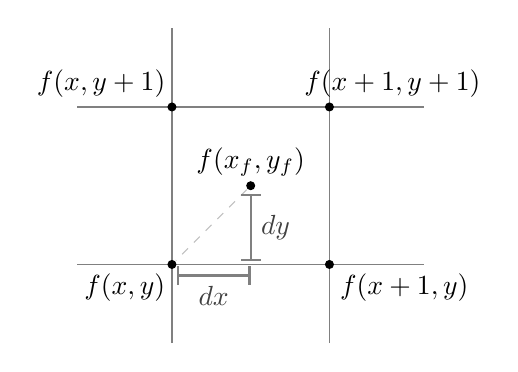
\begin{tikzpicture}
    \draw[step=\passo*2cm,color=gray] (-1.2*\passo,-1*\passo) grid (3.2*\passo,3*\passo);

    \node [fill,draw,circle,inner sep=1pt] at (0*\passo,0*\passo) {};
    \node at (-0.6*\passo,-0.3*\passo) {$f(x, y)$};
    \node [fill,draw,circle,inner sep=1pt] at (2*\passo,0*\passo) {};
    \node at (2.95*\passo,-0.3*\passo) {$f(x+1, y)$};
    \node [fill,draw,circle,inner sep=1pt] at (0*\passo,2*\passo) {};
    \node at (-0.9*\passo,2.3*\passo) {$f(x, y+1)$};
    \node [fill,draw,circle,inner sep=1pt] at (2*\passo,2*\passo) {};
    \node at (2.8*\passo,2.3*\passo) {$f(x+1, y+1)$};

    \node [fill,draw,circle,inner sep=1pt] at (1*\passo,1*\passo) {};
    \node at (1*\passo,1.3*\passo) {$f(x_f, y_f)$};

    \draw [color=lightgray,thin,dashed] (1*\passo - 0.05*\passo, 1 *\passo - 0.05*\passo) -- (0*\passo + 0.05*\passo, 0*\passo + 0.05*\passo);

    \draw [color=gray,thick,|-|] (1*\passo, 1 *\passo - 0.1*\passo) -- (1*\passo, 0*\passo + 0.04*\passo) node[midway, right, color=darkgray] {$dy$};
    \draw [color=gray,thick,|-|] (1*\passo - 0*\passo, -0.14 *\passo) -- (0*\passo + 0.06*\passo, -0.14*\passo) node[midway, below, color=darkgray] {$dx$};
\end{tikzpicture}

    \caption{Vizinhança de $(x_f, y_f)$.}
    \label{fig:viz:exemplo}
\end{figure}

Para pontos fora da figura, podemos usar a cor de fundo (escolhida como na \cref{sec:fundo}) como valor do pixel. Assim, $f(x, y) = z_\text{fundo}$ quando $x < 0$, $x \geq W_f$, $y < 0$ ou $y \geq H_f$.

\subsection{Pelo Vizinho Mais Próximo} \label{sec:interp:vizinho}

Nesse método, a intensidade da pixel é escolhido pelo vizinho com posição mais próxima de $(x_f, y_f)$. Assim: % TODO: formatação

\begin{align*}
    g(x_g, y_g) = f'(x_f, y_f) &= \begin{cases}
        f(x, y) & \text{se } dx < 0.5 \text{ e } dy < 0.5 \\
        f(x+1, y) & \text{se } dx \geq 0.5 \text{ e } dy < 0.5 \\
        f(x, y+1) & \text{se } dx < 0.5 \text{ e } dy \geq 0.5 \\
        f(x+1, y+1) & \text{se } dx \geq 0.5 \text{ e } dy \geq 0.5 \\
    \end{cases} \\
    &= f(\round(x_f), \round(y_f))
\end{align*}

\subsection{Bilinear} \label{sec:interp:bilinear}

\subsection{Bicúbica} \label{sec:interp:bicubica}

\subsection{Por Polinômios de Lagrange} \label{sec:interp:lagrange}
